\documentclass[aspectratio=169,10pt]{beamer}
\usepackage[T1]{fontenc}
\usepackage{amsmath,amssymb,amsfonts}
\usepackage{bm}
\usepackage{tikz}
\usepackage{xcolor}
\usetikzlibrary{arrows.meta,positioning,shapes,calc}

\definecolor{parchment}{HTML}{F4E8C8}
\definecolor{paper}{HTML}{FAF1D8}
\definecolor{ink}{HTML}{1A1A1A}
\definecolor{inkgray}{HTML}{5A5A5A}
\definecolor{accentred}{HTML}{8B1A1A}
\definecolor{accentgreen}{HTML}{2D5F2C}
\definecolor{accentblue}{HTML}{1F4E79}
\definecolor{redbg}{HTML}{F7E0DE}
\definecolor{grnbg}{HTML}{E0EBDC}
\definecolor{blubg}{HTML}{DDE6EF}
\definecolor{labelbg}{HTML}{EFE0B0}

\usefonttheme{serif}
\setbeamercolor{background canvas}{bg=parchment}
\setbeamercolor{normal text}{fg=ink}
\setbeamercolor{structure}{fg=ink}
\setbeamercolor{frametitle}{fg=ink,bg=parchment}
\setbeamercolor{title}{fg=ink}
\setbeamercolor{itemize item}{fg=ink}
\setbeamercolor{itemize subitem}{fg=ink}
\setbeamercolor{item}{fg=ink}
\setbeamercolor{caption name}{fg=ink}
\setbeamertemplate{navigation symbols}{}
\setbeamertemplate{itemize item}{\textbullet}

\setbeamertemplate{frametitle}{%
  \vspace{0.30em}%
  \begin{center}%
    {\bfseries\Large\insertframetitle\par}%
    \vspace{0.28em}%
    {\color{ink}\rule{0.86\paperwidth}{0.4pt}}%
  \end{center}%
  \vspace{0.10em}%
}
\setbeamertemplate{footline}{%
  \hbox to \paperwidth{\hfil\itshape\small\insertframenumber\hspace{0.7em}}%
  \vspace{0.35em}%
}

\newcommand{\vY}{\bm{Y}}
\newcommand{\vy}{\bm{y}}
\newcommand{\vA}{\bm{A}}
\newcommand{\vB}{\bm{B}}
\newcommand{\valpha}{\bm{\alpha}}
\newcommand{\vn}{\bm{n}}
\newcommand{\vs}{\bm{s}}
\newcommand{\vW}{\bm{W}}
\newcommand{\T}{^{\mathsf T}}
\newcommand{\Hh}{^{\mathsf H}}
\newcommand{\norm}[1]{\left\lVert #1\right\rVert}
\DeclareMathOperator*{\argmin}{arg\,min}

\tikzset{
  flowbox/.style={draw=ink,fill=paper,line width=0.6pt,
                  minimum width=2.5cm,minimum height=1.0cm,
                  align=center,font=\small\bfseries,inner sep=4pt},
  smallbox/.style={draw=ink,fill=paper,line width=0.4pt,
                   minimum width=0.7cm,minimum height=0.55cm,
                   inner sep=2pt,align=center,font=\footnotesize\itshape},
  method/.style={draw=accentgreen,fill=grnbg,line width=1.0pt,
                 align=center,font=\small\bfseries,inner sep=6pt},
  issue/.style={draw=accentred,fill=redbg,line width=1.0pt,
                align=center,font=\small\bfseries,inner sep=6pt},
  idea/.style={draw=accentblue,fill=blubg,line width=1.0pt,
               align=center,font=\small\bfseries,inner sep=6pt},
  flowarr/.style={-{Stealth[length=2.5mm,width=2mm]},line width=0.7pt},
  softarr/.style={-{Stealth[length=2mm,width=1.6mm]},line width=0.5pt,color=inkgray}
}

\newcommand{\bottomnote}[1]{%
  \begin{center}{\itshape\small #1}\end{center}}

\newcommand{\papercover}[4]{%
  \begin{frame}[plain]
    \vfill
    \begin{center}
      {\bfseries\Huge #1\par}
      \vspace{0.8cm}
      {\Large #2\par}
      \vspace{0.35cm}
      {\itshape\large\color{inkgray}#3\par}
      \vspace{0.55cm}
      {\small\texttt{\detokenize{#4}}\par}
    \end{center}
    \vfill
  \end{frame}}

\newcommand{\twocolmodel}[4]{%
  \begin{columns}[T,onlytextwidth]
    \begin{column}{0.48\textwidth}#1\end{column}
    \begin{column}{0.48\textwidth}#2\end{column}
  \end{columns}
  \bottomnote{#3\\#4}}


\begin{document}

\papercover
  {Partial FFT Demodulation}
  {Yerramalli, Stojanovic, and Mitra}
  {IEEE Transactions on Signal Processing, 2012}
  {partial_fft_doppler_ofdm.pdf}

\begin{frame}{1. Core problem}
\twocolmodel{
  \begin{itemize}\setlength{\itemsep}{0.45em}
    \item One full-symbol FFT averages a changing channel
    \item Subcarrier orthogonality breaks; ICI grows
    \item Full block equalization costly for large systems
  \end{itemize}
}{
  \[
    y_k=\int_0^T r(t)e^{-j2\pi f_k t}\,dt
  \]
  \[
    H(t)\;\text{varies inside }[0,T]
    \Rightarrow
    \text{ICI}
  \]
}{
  Replace one long FFT view with several short FFT views.
}{
  Short windows see less channel variation, and the branch outputs are recombined by weighting.
}
\end{frame}

\begin{frame}{2. Partial FFT observation}
\begin{center}
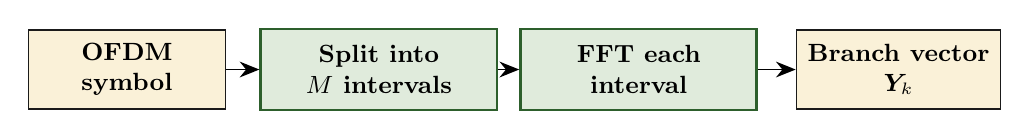
\begin{tikzpicture}[x=1cm,y=1cm]
  \node[flowbox] (sym) at (-5.0,0) {OFDM\\symbol};
  \node[method,minimum width=3.0cm] (split) at (-1.8,0) {Split into\\$M$ intervals};
  \node[method,minimum width=3.0cm] (fft) at (1.5,0) {FFT each\\interval};
  \node[flowbox] (vec) at (4.8,0) {Branch vector\\$\vY_k$};
  \draw[flowarr] (sym) -- (split);
  \draw[flowarr] (split) -- (fft);
  \draw[flowarr] (fft) -- (vec);
\end{tikzpicture}
\end{center}
\[
  \vY_k=
  \begin{bmatrix}
    Y_{k,1}&Y_{k,2}&\cdots&Y_{k,M}
  \end{bmatrix}^{\T},
  \qquad
  \widehat X_k=\vW_k\Hh\vY_k .
\]
\bottomnote{Equal weights collapse the branch vector back to the full FFT.\\The receiver behavior comes from the choice of branch weights.}
\end{frame}

\begin{frame}{3. Weight knowledge}
\begin{itemize}\setlength{\itemsep}{0.48em}
  \item Full channel knowledge: weights suppress ICI directly
  \item Partial knowledge: approximate statistics, reduced channel information
  \item No knowledge: weights learned from observations and pilots
  \item Complexity is moderate: $M$ branch values per carrier
\end{itemize}
\bottomnote{Although this paper is not by Wang or Zhou, \texttt{JUNA\_vs\_RPC} builds on its partial-FFT combiner.}
\end{frame}

\begin{frame}{4. JUNA connection}
\begin{itemize}\setlength{\itemsep}{0.5em}
  \item RPC collapses $\vY_k$ to a scalar using $\vW_k$
  \item JUNA keeps the branch vector and models which transmitted symbols generated it:
  \[
    \vY_k=\sum_{q\in\mathcal B(k)}\bm c_{kq}s_q+\vn_k .
  \]
  \item Partial FFT supplies the observation geometry
  \item JUNA changes the inference target
\end{itemize}
\bottomnote{\texttt{JUNA\_vs\_RPC.tex} builds on this change of inference target.}
\end{frame}

\end{document}
